\documentclass[12pt,a4paper]{article}

\usepackage[utf8]{inputenc}
\usepackage[T1]{fontenc}
\usepackage[italian]{babel}
\usepackage{geometry}
\usepackage{graphicx}
\usepackage{booktabs}
\usepackage{array}
\usepackage{float}
\usepackage{hyperref}
\usepackage{xcolor}
\usepackage{amsmath}
\usepackage{longtable}
\usepackage{caption}
\usepackage{subcaption}
\usepackage{enumitem}
\usepackage{listings}

\geometry{margin=2.45cm}
\setlength{\parskip}{0.55em}
\setlength{\parindent}{0pt}
\renewcommand{\arraystretch}{1.18}

\hypersetup{
    colorlinks=true,
    linkcolor=blue,
    urlcolor=blue,
    citecolor=blue
}

\lstdefinestyle{bashstyle}{
    basicstyle=\ttfamily\small,
    breaklines=true,
    frame=single,
    columns=fullflexible,
    backgroundcolor=\color{gray!8}
}
\lstset{style=bashstyle}

\title{\textbf{Domain Adaptation su MRI ADNI con CycleGAN}\\
\large Relazione tecnica del progetto}
\author{Gruppo: TBD \qquad Project ID: TBD}
\date{\today}

\begin{document}

\maketitle

\begin{abstract}
Questa relazione descrive il lavoro svolto per costruire una pipeline di domain adaptation su immagini di risonanza magnetica strutturale provenienti da ADNI. Il problema affrontato e' la variazione di dominio causata da scanner e produttori diversi: un classificatore addestrato su scansioni acquisite da un produttore puo' degradare quando viene valutato su immagini acquisite da un altro produttore. La pipeline implementata prepara volumi T1, costruisce split patient-level separando source e target domain per produttore, addestra un classificatore source-only, addestra una CycleGAN per tradurre lo stile delle immagini source verso il target, genera un training set aumentato e confronta le metriche finali sul target test set. Il codice e' stato organizzato secondo la struttura del repository: preprocessing in \texttt{src/datasets}, architetture in \texttt{src/models}, training in \texttt{src/training}, valutazione in \texttt{src/evaluation}, checkpoint in \texttt{experiments/checkpoints}, log in \texttt{experiments/logs} e figure in \texttt{figures}. I risultati ottenuti indicano che, nella configurazione eseguita, il baseline source-only raggiunge accuracy 0.7429 e macro-F1 0.7395 sul target test set, mentre il modello addestrato con dati aumentati tramite CycleGAN raggiunge accuracy 0.5714 e macro-F1 0.5585. La relazione discute quindi non solo l'implementazione, ma anche il fatto che l'adattamento generativo non ha migliorato la generalizzazione in questa run, probabilmente a causa della dimensione ridotta del dataset, dell'uso di sole slice centrali e della semplicita' delle architetture.
\end{abstract}

\tableofcontents
\newpage

\section{Introduzione}

La robustezza dei modelli di deep learning in ambito medico dipende in modo critico dalla qualita' e dall'omogeneita' dei dati di training. Nel caso delle immagini di risonanza magnetica, anche quando il protocollo clinico e' simile, le immagini possono cambiare sensibilmente in funzione del produttore dello scanner, della forza di campo, dei parametri di acquisizione e della pipeline di preprocessing. Questa variazione prende il nome di \emph{domain shift}: il modello apprende correlazioni statistiche sul dominio di addestramento, ma tali correlazioni possono non trasferirsi direttamente a un dominio di test differente.

Il progetto realizzato studia questo problema usando scansioni strutturali MRI del dataset ADNI. L'obiettivo pratico e' costruire una pipeline riproducibile che:

\begin{enumerate}[leftmargin=1.2cm]
    \item legge gli archivi MRI e i metadati IDA;
    \item filtra scansioni T1 e classi diagnostiche di interesse;
    \item costruisce split a livello paziente;
    \item considera il produttore dello scanner come dominio;
    \item addestra un classificatore source-only;
    \item addestra una CycleGAN per tradurre immagini dal dominio source al target;
    \item genera un training set aumentato;
    \item confronta quantitativamente e qualitativamente i risultati.
\end{enumerate}

La scelta di CycleGAN e' motivata dal fatto che il target domain viene usato senza supervisioni di classe nella fase di adattamento. In altre parole, la traduzione source-to-target puo' essere appresa da coppie non allineate di immagini source e target. Questo e' coerente con molti scenari reali di domain adaptation in cui si possiedono immagini non etichettate dal dominio target, ma non necessariamente annotazioni diagnostiche complete.

\section{Obiettivo del progetto}

L'obiettivo principale e' valutare se una traduzione di stile tra scanner, appresa con CycleGAN, possa migliorare la classificazione CN vs AD nel target domain rispetto a un baseline addestrato solo sul source domain. Il progetto non mira a proporre un modello clinico pronto all'uso, ma una pipeline sperimentale completa, verificabile e coerente con la struttura richiesta dal repository.

La domanda sperimentale puo' essere formulata come segue:

\begin{quote}
Dato un classificatore addestrato su MRI provenienti da scanner SIEMENS, l'aggiunta di slice source tradotte nello stile PHILIPS tramite CycleGAN migliora le prestazioni su un target test set PHILIPS?
\end{quote}

La risposta empirica, nella run attuale, e' negativa: il modello source-only e' risultato migliore del modello aumentato. Questo risultato e' comunque utile, perche' mostra una pipeline funzionante e mette in evidenza limiti tecnici e sperimentali importanti: numero ridotto di campioni, training generativo non supervisionato, uso di una sola slice centrale per volume, assenza di validazione qualitativa clinica e architetture volutamente leggere.

\section{Organizzazione del repository}

Durante il lavoro e' stata rispettata l'architettura del repository \texttt{dl26-projects}. Ogni cartella contiene componenti coerenti con il proprio README:

\begin{itemize}[leftmargin=1.2cm]
    \item \texttt{data/}: archivi ADNI, dati grezzi estratti e dati processati locali;
    \item \texttt{src/datasets/}: script di preparazione del dataset, split e costruzione del training set aumentato;
    \item \texttt{src/models/}: definizioni delle architetture PyTorch;
    \item \texttt{src/training/}: script di training e traduzione;
    \item \texttt{src/evaluation/}: metriche, confronto degli esperimenti e generazione figure;
    \item \texttt{experiments/configs/}: configurazioni sperimentali;
    \item \texttt{experiments/checkpoints/}: checkpoint addestrati;
    \item \texttt{experiments/logs/}: log CSV delle curve temporali;
    \item \texttt{experiments/outputs/}: metriche e output degli esperimenti;
    \item \texttt{figures/}: figure generate per analisi e relazione;
    \item \texttt{docs/}: report e documentazione finale.
\end{itemize}

Questa separazione evita di mischiare responsabilita' diverse. Le classi dei modelli non sono lasciate negli script di training, ma collocate in \texttt{src/models}. Le metriche e le figure non vengono prodotte manualmente, ma da uno script in \texttt{src/evaluation}. I checkpoint non sono salvati in \texttt{src/models}, perche' quella cartella contiene codice sorgente e non pesi addestrati.

\section{Dataset e dati utilizzati}

Il dataset utilizzato e' una selezione ADNI composta da scansioni MRI in formato NIfTI e metadati IDA in formato XML. Gli input locali usati dalla pipeline sono:

\begin{itemize}[leftmargin=1.2cm]
    \item \texttt{data/ADNI1\_Annual 2 Yr 3T.zip};
    \item \texttt{data/ADNI1\_Annual\_2\_Yr\_3T\_IDA\_Metadata.zip};
    \item \texttt{data/ADNI1\_Annual\_2\_Yr\_3T\_5\_26\_2026.csv}.
\end{itemize}

Il CSV di collezione contiene le colonne necessarie per associare ogni immagine al soggetto, al gruppo diagnostico, alla descrizione della scansione e alla data di acquisizione:

\begin{itemize}[leftmargin=1.2cm]
    \item \texttt{Image Data ID};
    \item \texttt{Subject};
    \item \texttt{Group};
    \item \texttt{Description};
    \item \texttt{Acq Date}.
\end{itemize}

Sono stati estratti 306 file \texttt{.nii} e 612 file \texttt{.xml}. Dopo il filtraggio per scansioni T1, field strength 3T e classi diagnostiche CN/AD, il dataset preparato contiene 173 volumi relativi a 52 soggetti.

\begin{table}[H]
\centering
\caption{Distribuzione dei dati preparati per produttore e classe.}
\begin{tabular}{lrr}
\toprule
Produttore & Disease & Healthy \\
\midrule
GE Medical Systems & 9 & 18 \\
Philips Medical Systems & 23 & 48 \\
Siemens & 26 & 49 \\
\midrule
Totale & 58 & 115 \\
\bottomrule
\end{tabular}
\end{table}

La tabella mostra che le classi sono sbilanciate verso \emph{healthy}; inoltre i produttori hanno numerosita' diverse. Questo influenza sia la stabilita' del training sia l'interpretazione delle metriche. Per questo motivo, oltre all'accuracy, viene riportata la macro-F1, che pesa le classi in modo piu' bilanciato.

\section{Preprocessing}

Il preprocessing e' implementato in \texttt{src/datasets/prepare\_adni.py}. Lo script svolge diverse operazioni:

\begin{enumerate}[leftmargin=1.2cm]
    \item legge il CSV di collezione ADNI;
    \item normalizza gli identificativi immagine;
    \item inferisce la modalita' dalla descrizione;
    \item filtra le scansioni T1;
    \item assegna l'etichetta diagnostica in modalita' \texttt{cn\_vs\_ad};
    \item collega il record CSV al file NIfTI e al file XML;
    \item estrae produttore, modello scanner, field strength e series UID dai metadati XML;
    \item normalizza il volume tramite min-max normalization;
    \item salva il volume come \texttt{.npy};
    \item produce \texttt{index\_prepared.csv}.
\end{enumerate}

Durante l'esecuzione iniziale e' emerso un collo di bottiglia: cercare ricorsivamente file NIfTI e XML per ogni riga del CSV era troppo lento. Lo script e' stato quindi ottimizzato indicizzando una sola volta tutti i file disponibili. Questa modifica riduce drasticamente il costo della fase di matching.

La normalizzazione min-max e' definita come:

\[
x' = \frac{x - \min(x)}{\max(x) - \min(x)}
\]

Quando il volume ha valore massimo uguale al minimo, viene restituito un volume nullo per evitare divisioni per zero.

\section{Split source e target}

Gli split sono creati con \texttt{src/datasets/make\_domain\_splits.py}. Il produttore dello scanner viene usato come dominio. Lo script sceglie automaticamente i due produttori piu' frequenti:

\begin{itemize}[leftmargin=1.2cm]
    \item source domain: \texttt{SIEMENS};
    \item target domain: \texttt{PHILIPS MEDICAL SYSTEMS}.
\end{itemize}

Lo split e' patient-level: un soggetto non deve comparire contemporaneamente in training e test. Questa scelta e' essenziale per evitare leakage, perche' piu' scansioni dello stesso soggetto possono essere molto simili e rendere il task artificialmente piu' semplice.

\begin{table}[H]
\centering
\caption{Split patient-level usati nella pipeline.}
\begin{tabular}{lrrr}
\toprule
Split & Scansioni & Soggetti & Dominio \\
\midrule
Source train & 58 & 17 & Siemens \\
Source validation & 17 & 5 & Siemens \\
Target adaptation unlabeled & 36 & 10 & Philips \\
Target test & 35 & 11 & Philips \\
\bottomrule
\end{tabular}
\end{table}

La parte target adaptation viene usata per addestrare la CycleGAN come dominio target non etichettato. Il target test set viene mantenuto separato e usato solo per la valutazione finale dei classificatori.

\section{Architetture implementate}

Le architetture sono state collocate in \texttt{src/models}, in accordo con il README della cartella.

\subsection{Classificatore CNN}

Il classificatore e' definito in \texttt{src/models/classifier.py}. Si tratta di una CNN leggera che opera su slice 2D monocanale estratte dal centro del volume MRI. La rete e' composta da:

\begin{itemize}[leftmargin=1.2cm]
    \item tre blocchi convolutional con batch normalization e ReLU;
    \item max pooling nei primi due blocchi;
    \item adaptive average pooling a dimensione fissa;
    \item fully connected layer da 128 unita';
    \item dropout;
    \item layer di output a due classi.
\end{itemize}

L'uso di una rete leggera e' stato scelto per rendere il training praticabile localmente e per mantenere la pipeline semplice. Il limite principale e' che una singola slice centrale non rappresenta tutta l'informazione volumetrica del cervello. Un miglioramento naturale sarebbe passare a modelli 2.5D o 3D.

\subsection{CycleGAN}

La CycleGAN e' definita in \texttt{src/models/cyclegan.py}. Sono presenti due componenti:

\begin{itemize}[leftmargin=1.2cm]
    \item \texttt{Generator}: traduce immagini da un dominio all'altro;
    \item \texttt{Discriminator}: distingue immagini reali da immagini generate.
\end{itemize}

Durante il training vengono usati due generatori:

\[
G_{S \rightarrow T}
\]

\[
G_{T \rightarrow S}
\]

e due discriminatori, uno per il source domain e uno per il target domain. La loss totale del generatore include:

\begin{itemize}[leftmargin=1.2cm]
    \item adversarial loss;
    \item cycle-consistency loss;
    \item identity loss.
\end{itemize}

La cycle-consistency impone che una immagine source tradotta nel target e poi riportata nel source rimanga coerente:

\[
G_{T \rightarrow S}(G_{S \rightarrow T}(x_S)) \approx x_S
\]

Analogamente per il target:

\[
G_{S \rightarrow T}(G_{T \rightarrow S}(x_T)) \approx x_T
\]

\section{Problemi tecnici risolti durante lo sviluppo}

Durante l'esecuzione della pipeline sono emersi diversi problemi pratici.

\subsection{Dipendenza NIfTI}

Il sistema inizialmente non aveva \texttt{nibabel}, libreria necessaria per caricare i file NIfTI. La dipendenza e' stata installata e verificata. Dopo l'installazione, \texttt{prepare\_adni.py} e' stato in grado di leggere i volumi e salvarli in formato NumPy.

\subsection{Dimensioni diverse delle slice}

Il training del classificatore si e' inizialmente fermato perche' alcune slice avevano dimensioni diverse, ad esempio \texttt{240x256} e \texttt{256x256}. PyTorch non puo' creare batch con tensori di dimensioni diverse. Il problema e' stato risolto aggiungendo un resize bilineare a \texttt{256x256} nei dataset usati da classificatore, CycleGAN e traduzione.

\subsection{Caricamento lento dei volumi}

Un altro collo di bottiglia era il caricamento dell'intero volume 3D solo per estrarre una slice centrale. Lo script e' stato ottimizzato usando \texttt{np.load(..., mmap\_mode="r")}, cosi' da ridurre il carico di I/O.

\subsection{Separazione delle responsabilita'}

Inizialmente alcune definizioni modello erano dentro gli script di training. Per allineare il progetto al README di \texttt{src/models}, le architetture sono state spostate in file dedicati e importate dagli script di training.

\section{Pipeline sperimentale}

La pipeline eseguita e' composta da otto fasi principali.

\subsection{Estrazione dati}

Gli archivi sono stati estratti in:

\begin{lstlisting}[language=bash]
data/raw/nifti
data/raw/metadata
\end{lstlisting}

Il conteggio finale e' stato:

\begin{itemize}[leftmargin=1.2cm]
    \item 306 file NIfTI;
    \item 612 file XML.
\end{itemize}

\subsection{Preparazione volumi}

\begin{lstlisting}[language=bash]
python src/datasets/prepare_adni.py \
  --csv data/ADNI1_Annual_2_Yr_3T_5_26_2026.csv \
  --nifti-root data/raw/nifti \
  --metadata-root data/raw/metadata \
  --out-dir data/processed/00_prepared \
  --field 3T \
  --label-mode cn_vs_ad
\end{lstlisting}

Il risultato principale e':

\begin{lstlisting}
data/processed/00_prepared/index_prepared.csv
\end{lstlisting}

\subsection{Split domini}

\begin{lstlisting}[language=bash]
python src/datasets/make_domain_splits.py \
  --index-csv data/processed/00_prepared/index_prepared.csv \
  --out-dir data/processed/01_domain_split
\end{lstlisting}

\subsection{Training baseline source-only}

\begin{lstlisting}[language=bash]
python src/training/train_classifier.py \
  --train-csv data/processed/01_domain_split/source_train.csv \
  --val-csv data/processed/01_domain_split/source_val.csv \
  --test-csv data/processed/01_domain_split/target_test.csv \
  --out-dir experiments/outputs/classifier_source_only \
  --checkpoint-dir experiments/checkpoints \
  --checkpoint-name classifier_source_only_best_model.pt \
  --epochs 20 \
  --batch-size 8
\end{lstlisting}

\subsection{Training CycleGAN}

\begin{lstlisting}[language=bash]
python src/training/train_cyclegan.py \
  --source-csv data/processed/01_domain_split/source_train.csv \
  --target-csv data/processed/01_domain_split/target_adapt_unlabeled.csv \
  --out-dir experiments/outputs/cyclegan_scanner \
  --checkpoint-dir experiments/checkpoints \
  --epochs 30 \
  --batch-size 4
\end{lstlisting}

\subsection{Traduzione source-to-target}

\begin{lstlisting}[language=bash]
python -m src.training.translate_source \
  --source-csv data/processed/01_domain_split/source_train.csv \
  --generator experiments/checkpoints/cyclegan_generator_source_to_target.pt \
  --out-dir data/processed/02_translated_source
\end{lstlisting}

\subsection{Training set aumentato}

\begin{lstlisting}[language=bash]
python src/datasets/build_augmented_train.py \
  --source-csv data/processed/01_domain_split/source_train.csv \
  --translated-csv data/processed/02_translated_source/translated_source_train.csv \
  --out-csv data/processed/02_translated_source/source_train_augmented.csv
\end{lstlisting}

Il training set aumentato contiene 116 righe: 58 esempi source originali e 58 slice tradotte.

\subsection{Training classificatore aumentato}

\begin{lstlisting}[language=bash]
python src/training/train_classifier.py \
  --train-csv data/processed/02_translated_source/source_train_augmented.csv \
  --val-csv data/processed/01_domain_split/source_val.csv \
  --test-csv data/processed/01_domain_split/target_test.csv \
  --out-dir experiments/outputs/classifier_cyclegan_augmented \
  --checkpoint-dir experiments/checkpoints \
  --checkpoint-name classifier_cyclegan_augmented_best_model.pt \
  --epochs 20 \
  --batch-size 8
\end{lstlisting}

\section{Valutazione}

La valutazione e' implementata in \texttt{src/evaluation/evaluate\_pipeline.py}. Lo script confronta i file \texttt{metrics.json} dei due classificatori e produce:

\begin{itemize}[leftmargin=1.2cm]
    \item \texttt{experiments/outputs/evaluation/summary.csv};
    \item \texttt{experiments/outputs/evaluation/summary.json};
    \item \texttt{experiments/outputs/evaluation/summary.md};
    \item figure in \texttt{figures/}.
\end{itemize}

Le metriche principali sono accuracy e macro-F1. La macro-F1 e' particolarmente utile nel contesto attuale perche' il target test set contiene 12 campioni disease e 23 campioni healthy.

\section{Risultati quantitativi}

\begin{table}[H]
\centering
\caption{Confronto finale sul target test set Philips.}
\begin{tabular}{lrrrr}
\toprule
Modello & Accuracy & Macro-F1 & Delta Accuracy & Delta Macro-F1 \\
\midrule
Source-only & 0.7429 & 0.7395 & 0.0000 & 0.0000 \\
CycleGAN-augmented & 0.5714 & 0.5585 & -0.1714 & -0.1810 \\
\bottomrule
\end{tabular}
\end{table}

Il baseline source-only supera il modello aumentato sia in accuracy sia in macro-F1. In particolare, la differenza e':

\[
\Delta Accuracy = -0.1714
\]

\[
\Delta MacroF1 = -0.1810
\]

Questo significa che, nella configurazione eseguita, l'aggiunta delle immagini tradotte non ha aiutato la generalizzazione verso il target domain.

\begin{table}[H]
\centering
\caption{Metriche per classe del modello source-only. Classe 0: disease, classe 1: healthy.}
\begin{tabular}{lrrrr}
\toprule
Classe & Precision & Recall & F1-score & Support \\
\midrule
Disease & 0.5789 & 0.9167 & 0.7097 & 12 \\
Healthy & 0.9375 & 0.6522 & 0.7692 & 23 \\
\midrule
Macro avg & 0.7582 & 0.7844 & 0.7395 & 35 \\
\bottomrule
\end{tabular}
\end{table}

\begin{table}[H]
\centering
\caption{Metriche per classe del modello CycleGAN-augmented. Classe 0: disease, classe 1: healthy.}
\begin{tabular}{lrrrr}
\toprule
Classe & Precision & Recall & F1-score & Support \\
\midrule
Disease & 0.4118 & 0.5833 & 0.4828 & 12 \\
Healthy & 0.7222 & 0.5652 & 0.6341 & 23 \\
\midrule
Macro avg & 0.5670 & 0.5743 & 0.5585 & 35 \\
\bottomrule
\end{tabular}
\end{table}

\section{Scatterplot delle metriche}

La Figura~\ref{fig:scatter} mostra il confronto fra accuracy e macro-F1. La posizione del modello source-only e' piu' vicina all'angolo alto a destra, indicando prestazioni migliori su entrambe le metriche.

\begin{figure}[H]
    \centering
    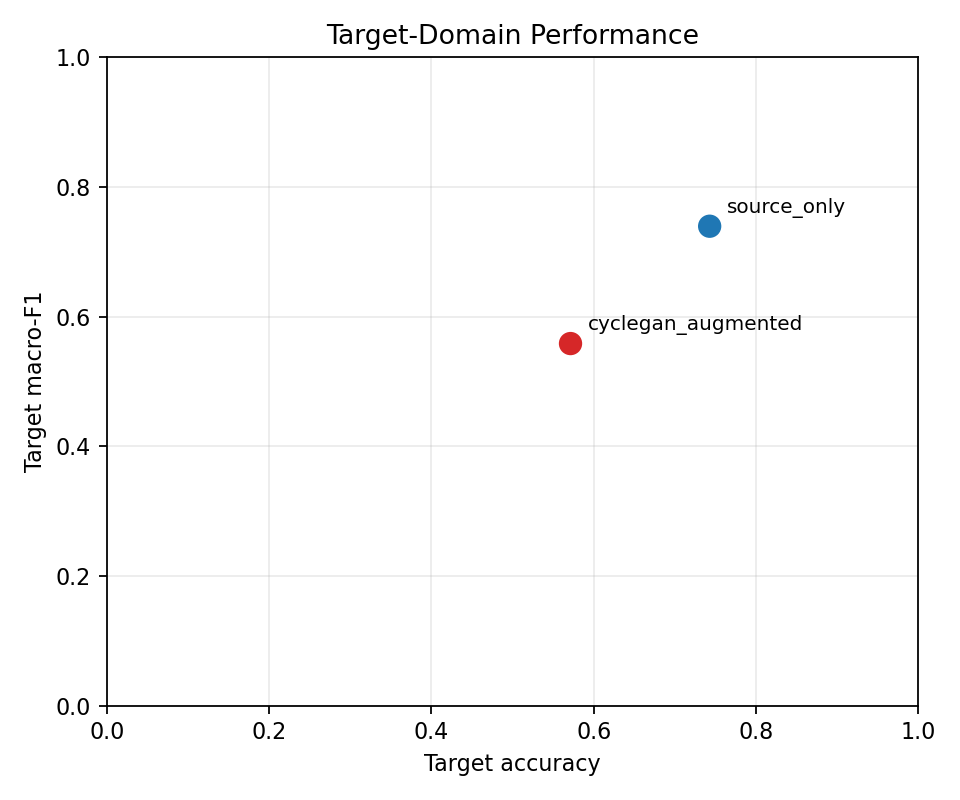
\includegraphics[width=0.72\textwidth]{../figures/metric_scatter_accuracy_f1.png}
    \caption{Scatterplot accuracy/macro-F1 dei due modelli valutati sul target test set.}
    \label{fig:scatter}
\end{figure}

\section{Curve temporali del classificatore}

La Figura~\ref{fig:classifier_curves} confronta loss, validation accuracy e validation macro-F1 dei due training del classificatore. La curva source-only mostra una maggiore instabilita' nelle epoche intermedie ma raggiunge picchi di validazione piu' alti. Il modello aumentato raggiunge un massimo di validation macro-F1 pari a 0.7424 alla sedicesima epoca, ma non trasferisce questo vantaggio al target test set.

\begin{figure}[H]
    \centering
    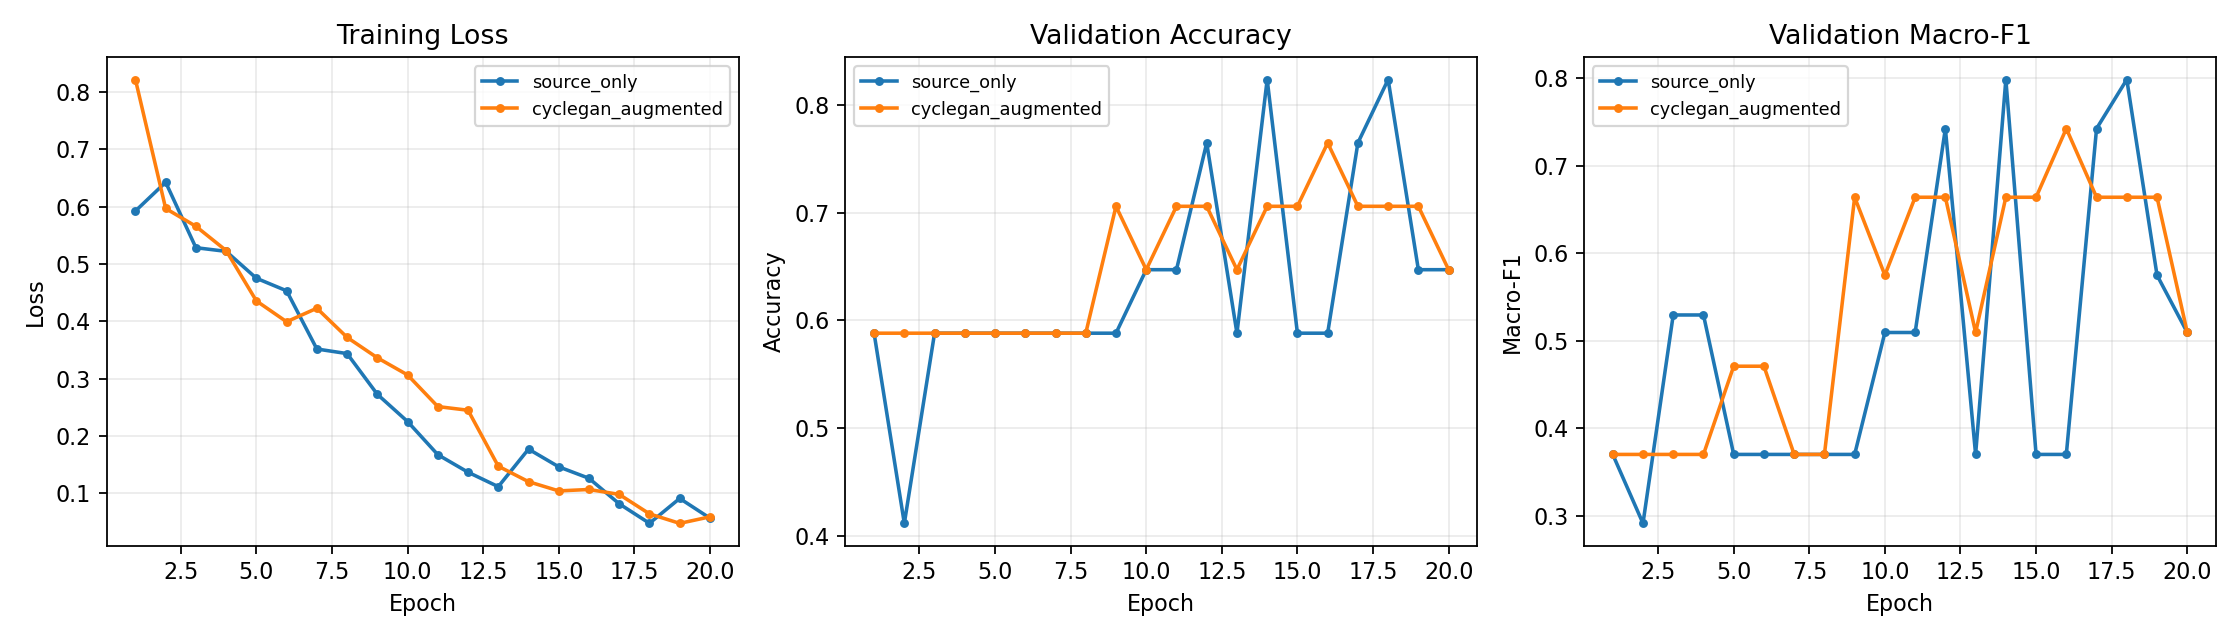
\includegraphics[width=\textwidth]{../figures/classifier_temporal_metrics.png}
    \caption{Curve temporali di loss, validation accuracy e validation macro-F1 per source-only e CycleGAN-augmented.}
    \label{fig:classifier_curves}
\end{figure}

Una possibile interpretazione e' che la validazione, essendo ancora nel source domain Siemens, non misura direttamente il miglioramento sul target Philips. Il modello puo' apparire buono in validazione source ma non necessariamente generalizzare al target.

\section{Curve temporali della CycleGAN}

La Figura~\ref{fig:cyclegan_curves} mostra le loss del generatore e del discriminatore durante le 30 epoche di CycleGAN. La generator loss scende rapidamente nelle prime epoche, passando da circa 3.28 a valori intorno a 1.0. La discriminator loss rimane invece relativamente stabile.

\begin{figure}[H]
    \centering
    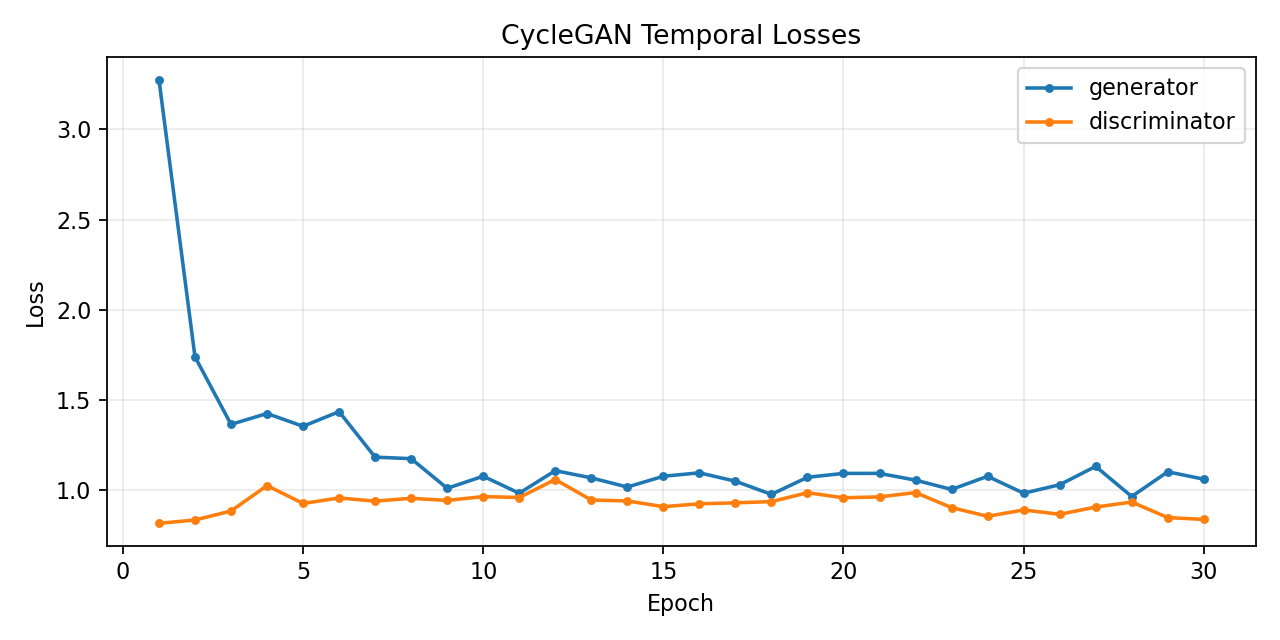
\includegraphics[width=0.88\textwidth]{../figures/cyclegan_temporal_losses.png}
    \caption{Loss generator/discriminator della CycleGAN durante il training.}
    \label{fig:cyclegan_curves}
\end{figure}

La stabilita' numerica della loss non implica automaticamente che la traduzione sia utile per la classificazione. Una CycleGAN puo' produrre immagini visivamente plausibili ma rimuovere o alterare dettagli discriminativi. Nel contesto medico questo e' un rischio importante.

\section{Preview qualitative delle immagini modificate}

La Figura~\ref{fig:qualitative} mostra esempi qualitativi di slice source originali, slice tradotte e differenza assoluta. Queste immagini consentono di verificare se il generatore produce modifiche visibili e dove esse si concentrano.

\begin{figure}[H]
    \centering
    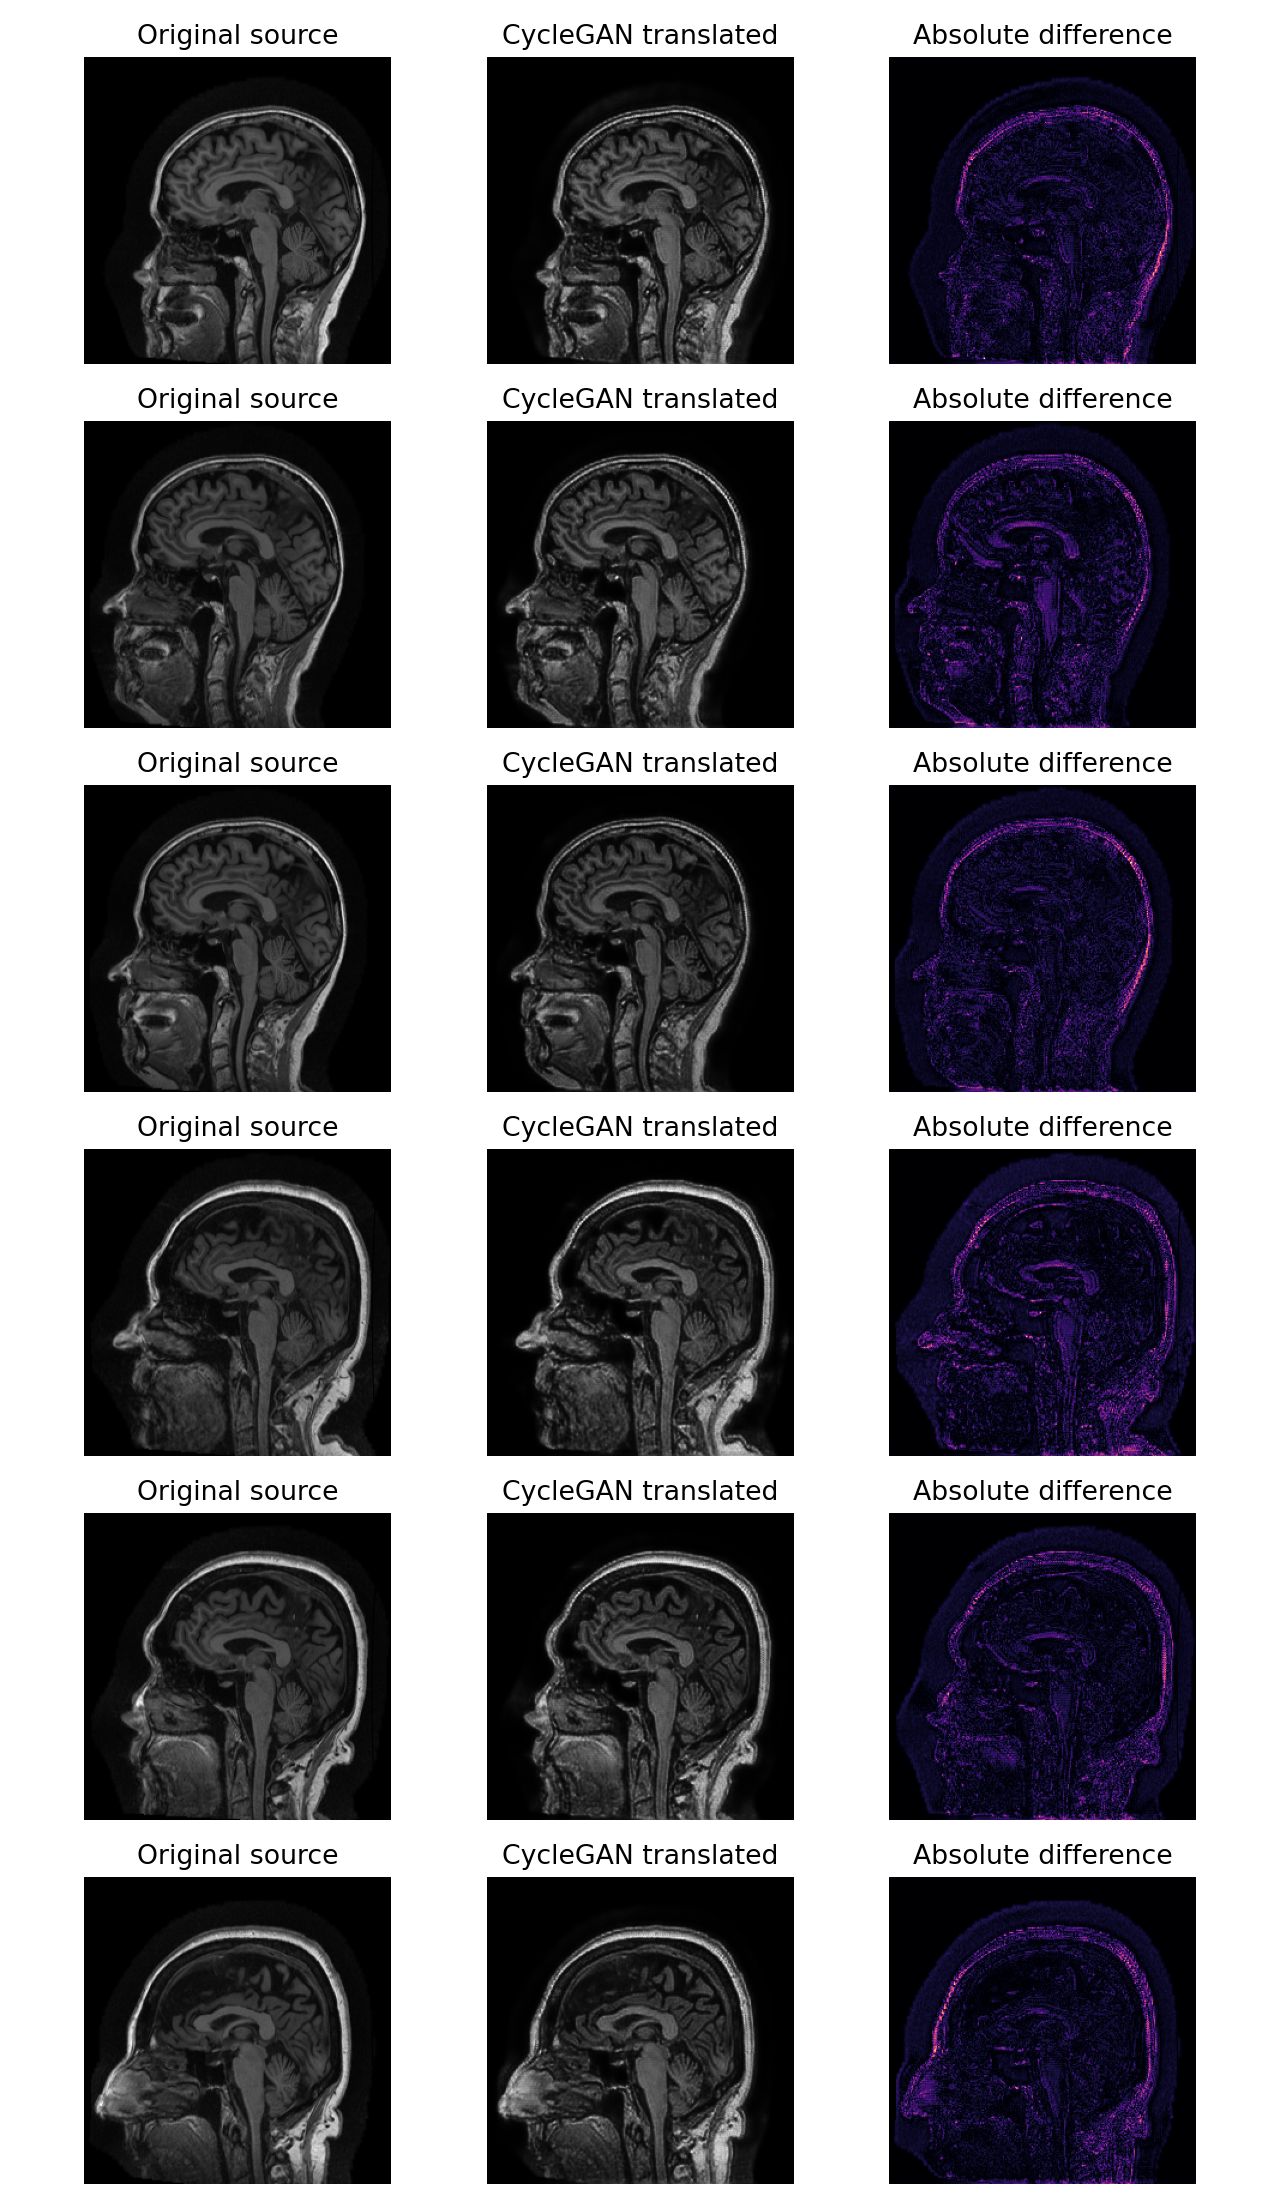
\includegraphics[width=0.82\textwidth]{../figures/qualitative_translation_previews.png}
    \caption{Preview qualitative: originale source, traduzione CycleGAN e differenza assoluta.}
    \label{fig:qualitative}
\end{figure}

Le differenze assolute mostrano che la trasformazione modifica la distribuzione visuale delle slice. Tuttavia, l'effetto non garantisce un miglioramento diagnostico. Per un uso piu' rigoroso sarebbe necessario controllare che la traduzione preservi strutture anatomiche e non introduca artefatti.

\section{Discussione dei risultati}

Il risultato principale e' che il baseline source-only ha ottenuto prestazioni migliori del modello CycleGAN-augmented. Questo puo' sembrare controintuitivo, perche' l'adattamento di dominio dovrebbe teoricamente ridurre il gap fra Siemens e Philips. Tuttavia, ci sono varie ragioni tecniche per cui cio' puo' accadere.

Primo, il dataset e' piccolo. Il source train contiene 58 scansioni, e il target adaptation set 36 scansioni. Per addestrare una CycleGAN, questi numeri sono molto limitati. Il modello generativo puo' imparare trasformazioni superficiali o instabili invece di una vera mappatura robusta fra domini.

Secondo, la pipeline usa solo la slice centrale di ogni volume. Questa scelta rende il training piu' leggero, ma riduce drasticamente l'informazione anatomica. La diagnosi CN vs AD puo' dipendere da pattern volumetrici distribuiti, non sempre visibili nella sola slice centrale.

Terzo, le immagini generate vengono usate come augmentation accanto agli originali, ma non c'e' una selezione qualitativa o quantitativa delle traduzioni. Se alcune immagini tradotte contengono artefatti, il classificatore puo' apprendere segnali non utili.

Quarto, la validazione del classificatore viene fatta su \texttt{source\_val}, quindi su Siemens. Questo puo' favorire il modello source-only e non fornire una stima diretta delle prestazioni target. Una possibile estensione sarebbe usare una piccola porzione target etichettata come validation, se disponibile e coerente con il protocollo sperimentale.

Quinto, la CycleGAN non e' vincolata da una loss diagnostica. Essa ottimizza plausibilita' visuale e consistenza ciclica, ma non necessariamente preserva caratteristiche legate alla malattia. In ambito medico, questa distinzione e' cruciale.

\section{Checkpoint e artefatti prodotti}

I checkpoint sono stati salvati in \texttt{experiments/checkpoints}, come richiesto dal README della cartella:

\begin{itemize}[leftmargin=1.2cm]
    \item \texttt{classifier\_source\_only\_best\_model.pt};
    \item \texttt{classifier\_source\_only\_best\_model\_labels.json};
    \item \texttt{cyclegan\_generator\_source\_to\_target.pt};
    \item \texttt{cyclegan\_generator\_target\_to\_source.pt};
    \item \texttt{classifier\_cyclegan\_augmented\_best\_model.pt};
    \item \texttt{classifier\_cyclegan\_augmented\_best\_model\_labels.json}.
\end{itemize}

I log delle curve sono stati salvati in \texttt{experiments/logs}:

\begin{itemize}[leftmargin=1.2cm]
    \item \texttt{classifier\_source\_only\_history.csv};
    \item \texttt{classifier\_cyclegan\_augmented\_history.csv};
    \item \texttt{cyclegan\_scanner\_history.csv}.
\end{itemize}

Le figure sono state salvate in \texttt{figures}:

\begin{itemize}[leftmargin=1.2cm]
    \item \texttt{metric\_scatter\_accuracy\_f1.png};
    \item \texttt{classifier\_temporal\_metrics.png};
    \item \texttt{cyclegan\_temporal\_losses.png};
    \item \texttt{qualitative\_translation\_previews.png}.
\end{itemize}

\section{Riproducibilita'}

La configurazione della pipeline e' stata salvata in:

\begin{lstlisting}
experiments/configs/adni_cyclegan_pipeline.json
\end{lstlisting}

Il file contiene path, iperparametri e directory di output. I principali iperparametri sono:

\begin{table}[H]
\centering
\caption{Iperparametri principali.}
\begin{tabular}{lr}
\toprule
Parametro & Valore \\
\midrule
Classifier epochs & 20 \\
Classifier batch size & 8 \\
Classifier learning rate & 0.001 \\
CycleGAN epochs & 30 \\
CycleGAN batch size & 4 \\
CycleGAN learning rate & 0.0002 \\
Cycle consistency weight & 10.0 \\
Identity weight & 2.0 \\
\bottomrule
\end{tabular}
\end{table}

Per riprodurre la pipeline completa, l'ordine corretto e':

\begin{enumerate}[leftmargin=1.2cm]
    \item estrazione archivi in \texttt{data/raw};
    \item preparazione ADNI;
    \item split source/target;
    \item training source-only;
    \item training CycleGAN;
    \item traduzione source;
    \item costruzione training set aumentato;
    \item training classificatore aumentato;
    \item evaluation e generazione figure.
\end{enumerate}

\section{Limiti}

Il progetto presenta diversi limiti che devono essere chiariti.

\subsection{Dimensione del dataset}

Il numero di campioni e' ridotto. In particolare, il target test set contiene solo 35 scansioni. Questo rende le metriche sensibili a poche predizioni sbagliate.

\subsection{Uso di slice 2D}

La pipeline usa la slice centrale del volume, non tutto il volume 3D. Questo semplifica il training ma limita fortemente la rappresentazione anatomica.

\subsection{CycleGAN non supervisionata}

La CycleGAN non riceve informazione diagnostica. Essa puo' imparare trasformazioni di intensita' o texture che non sono necessariamente utili alla classificazione.

\subsection{Valutazione qualitativa non clinica}

Le preview qualitative mostrano differenze visive, ma non costituiscono una validazione clinica. Per un progetto medico reale servirebbe un controllo piu' approfondito degli artefatti.

\subsection{Assenza di confronti multipli}

La pipeline e' stata eseguita con una configurazione principale. Non sono state ancora effettuate ablation su seed, produttori, batch size, numero di epoche, architettura o loss.

\section{Possibili estensioni}

Le estensioni piu' utili sono:

\begin{itemize}[leftmargin=1.2cm]
    \item usare modelli 3D o 2.5D invece della sola slice centrale;
    \item aggiungere data augmentation geometrica e di intensita';
    \item usare una validazione target etichettata se disponibile;
    \item confrontare CycleGAN con metodi di feature-level adaptation;
    \item aggiungere metriche di qualita' delle immagini generate;
    \item visualizzare embedding prima e dopo adattamento;
    \item eseguire piu' seed e riportare media e deviazione standard;
    \item usare scanner GE come ulteriore dominio di test;
    \item introdurre early stopping basato su una metrica piu' coerente con il target domain.
\end{itemize}

\section{Conclusione}

Il progetto ha prodotto una pipeline completa e riproducibile per studiare domain adaptation su MRI ADNI. Sono stati implementati preprocessing, split patient-level per dominio scanner, classificatore baseline, CycleGAN, traduzione source-to-target, training aumentato, evaluation quantitativa e figure qualitative.

Il risultato finale e' che il modello source-only ha ottenuto performance superiori al modello CycleGAN-augmented sul target test set Philips. Questo non invalida la pipeline: al contrario, fornisce un risultato sperimentale chiaro e utile. La traduzione generativa, nella configurazione attuale, non e' sufficiente a migliorare la classificazione. La causa piu' probabile e' la combinazione di dataset piccolo, uso di sole slice centrali e training CycleGAN non supervisionato rispetto al task diagnostico.

Il lavoro svolto costituisce quindi una base solida per esperimenti successivi. La struttura del codice e' stata organizzata secondo le responsabilita' del repository, gli artefatti sono stati salvati nelle cartelle corrette e le figure richieste sono generate automaticamente dallo script di evaluation.

\newpage
\appendix

\section{Comandi principali}

\begin{lstlisting}[language=bash]
python src/datasets/prepare_adni.py \
  --csv data/ADNI1_Annual_2_Yr_3T_5_26_2026.csv \
  --nifti-root data/raw/nifti \
  --metadata-root data/raw/metadata \
  --out-dir data/processed/00_prepared \
  --field 3T \
  --label-mode cn_vs_ad

python src/datasets/make_domain_splits.py \
  --index-csv data/processed/00_prepared/index_prepared.csv \
  --out-dir data/processed/01_domain_split

python src/training/train_classifier.py \
  --train-csv data/processed/01_domain_split/source_train.csv \
  --val-csv data/processed/01_domain_split/source_val.csv \
  --test-csv data/processed/01_domain_split/target_test.csv \
  --out-dir experiments/outputs/classifier_source_only \
  --checkpoint-dir experiments/checkpoints \
  --checkpoint-name classifier_source_only_best_model.pt

python src/training/train_cyclegan.py \
  --source-csv data/processed/01_domain_split/source_train.csv \
  --target-csv data/processed/01_domain_split/target_adapt_unlabeled.csv \
  --out-dir experiments/outputs/cyclegan_scanner \
  --checkpoint-dir experiments/checkpoints

python -m src.training.translate_source \
  --source-csv data/processed/01_domain_split/source_train.csv \
  --generator experiments/checkpoints/cyclegan_generator_source_to_target.pt \
  --out-dir data/processed/02_translated_source

python src/datasets/build_augmented_train.py \
  --source-csv data/processed/01_domain_split/source_train.csv \
  --translated-csv data/processed/02_translated_source/translated_source_train.csv \
  --out-csv data/processed/02_translated_source/source_train_augmented.csv

python src/training/train_classifier.py \
  --train-csv data/processed/02_translated_source/source_train_augmented.csv \
  --val-csv data/processed/01_domain_split/source_val.csv \
  --test-csv data/processed/01_domain_split/target_test.csv \
  --out-dir experiments/outputs/classifier_cyclegan_augmented \
  --checkpoint-dir experiments/checkpoints \
  --checkpoint-name classifier_cyclegan_augmented_best_model.pt

python src/evaluation/evaluate_pipeline.py \
  --baseline experiments/outputs/classifier_source_only/metrics.json \
  --augmented experiments/outputs/classifier_cyclegan_augmented/metrics.json \
  --out-dir experiments/outputs/evaluation \
  --figures-dir figures
\end{lstlisting}

\section{Dichiarazione sull'uso di strumenti AI}

Durante lo sviluppo sono stati usati strumenti di assistenza AI per supportare attivita' di debugging, generazione di boilerplate, documentazione tecnica e organizzazione della relazione. Le decisioni progettuali, l'esecuzione degli esperimenti e la responsabilita' del risultato rimangono a carico del gruppo.

\begin{thebibliography}{9}

\bibitem{cyclegan}
Zhu, J.-Y., Park, T., Isola, P., Efros, A. A.
\textit{Unpaired Image-to-Image Translation using Cycle-Consistent Adversarial Networks}.
ICCV, 2017.

\bibitem{adni}
Alzheimer's Disease Neuroimaging Initiative.
\textit{ADNI: Alzheimer's Disease Neuroimaging Initiative}.

\bibitem{domainadaptation}
Ganin, Y., et al.
\textit{Domain-Adversarial Training of Neural Networks}.
Journal of Machine Learning Research, 2016.

\end{thebibliography}

\end{document}
